\documentclass[]{article}
\usepackage[round]{natbib}

\usepackage{fullpage}
\usepackage{listings}
\usepackage{url}
\usepackage{authblk}
\usepackage{graphicx}
\usepackage{color}

% lorem ipsum dummy text
\usepackage{lipsum}

\lstset{language=Python}

% local definitions
\newcommand{\comment}[1]{{\textcolor{red}{Comment: #1}}}

% cross-reference with supplement
\usepackage{xr}
\externaldocument{supplement}

\begin{document}

\title{An article template}
\author[1,*]{The Author}
\affil[1]{Planet Earth}
\affil[*]{email@address.edu}
\maketitle

\abstract{
A very simple template for an article class document.
}

\section{Introduction}

There are a few sections below.

\lipsum[2-4]

\section{Code blocks}

A python snippet:
\begin{lstlisting}[frame=single]
dbg = msprime.DemographyDebugger(
  population_configurations=population_configurations,
  migration_matrix=migration_matrix,
  demographic_events=demographic_events)
dbg.print_history()
ts = msprime.simulate(
  population_configurations=population_configurations,
  migration_matrix=migration_matrix,
  demographic_events=demographic_events)
\end{lstlisting}
or
\begin{lstlisting}[frame=single]
dbg = demography.debug()
dbg.print_history()
ts = msprime.simulate(demography=demography)
\end{lstlisting}

This was in discussion of \citet{kelleher2016efficient}.
\section{Figures}

Place figures below, where you can see Fig.~\ref{fig:1}:

\begin{figure}[ht]
\begin{center}
\makebox[\textwidth][c]{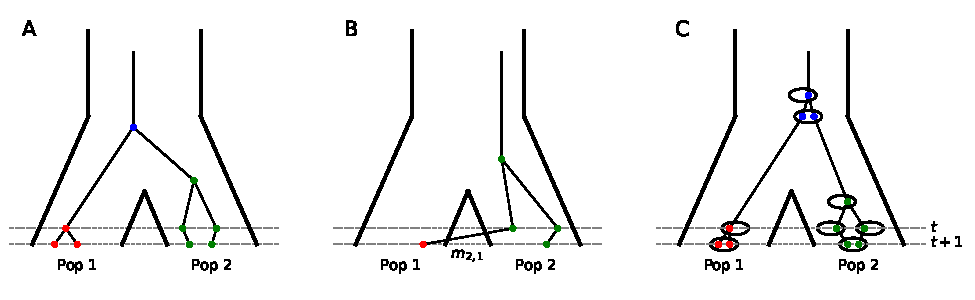
\includegraphics{figures/fig1.pdf}}
\caption{\textbf{The first figure}.
    It has a caption.
}
\label{fig:1}
\end{center}
\end{figure}

\lipsum[1]

We can even reference a table in the supplement, say Table~\ref{tab:1kgpops}.

\break

\bibliographystyle{plainnat}
\bibliography{paper}

\break

\renewcommand{\theequation}{A\arabic{equation}}
\renewcommand{\thefigure}{A\arabic{figure}}
\renewcommand{\thetable}{A\arabic{table}}
\setcounter{figure}{0}
\setcounter{equation}{0}
\setcounter{table}{0}

\appendix
\renewcommand{\thesection}{A\arabic{section}}

\section{Appendix} \label{appendix}

This is in the appendix. There is a figure (Fig.~\ref{fig:A1}) below.

\lipsum[1-3]

\begin{figure}[ht]
\begin{center}
\makebox[\textwidth][c]{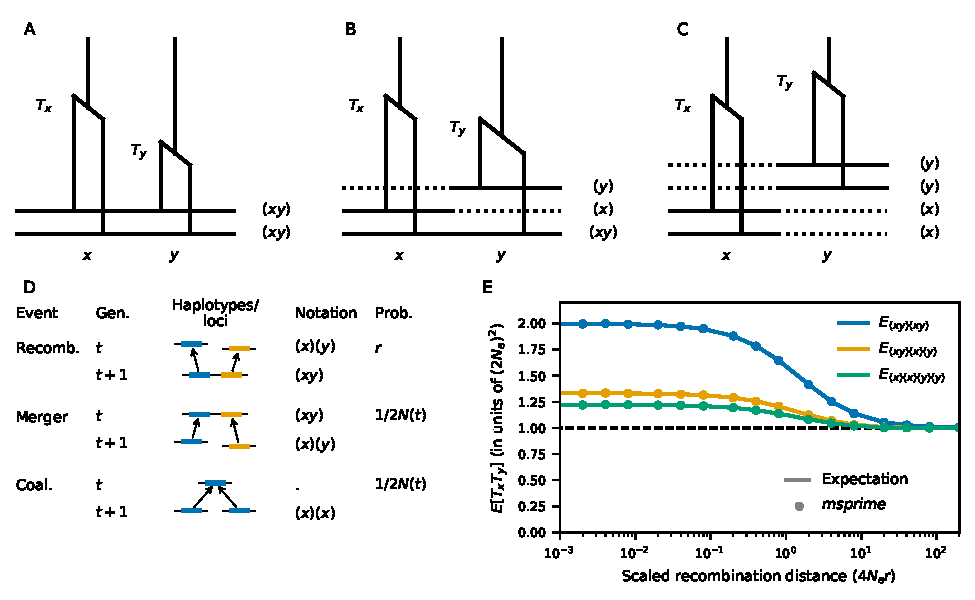
\includegraphics{figures/fig2.pdf}}
\caption{\textbf{A figure in the appendix.}.
}
\label{fig:A1}
\end{center}
\end{figure}

\end{document}
